\documentclass[review]{elsarticle}

\usepackage{lineno,hyperref}
\modulolinenumbers[5]

\journal{Journal of Pathology Informatics}

%%%%%%%%%%%%%%%%%%%%%%%
%% Elsevier bibliography styles
%%%%%%%%%%%%%%%%%%%%%%%
%% To change the style, put a % in front of the second line of the current style and
%% remove the % from the second line of the style you would like to use.
%%%%%%%%%%%%%%%%%%%%%%%

%% Numbered
%\bibliographystyle{model1-num-names}

%% Numbered without titles
%\bibliographystyle{model1a-num-names}

%% Harvard
%\bibliographystyle{model2-names.bst}\biboptions{authoryear}

%% Vancouver numbered
%\usepackage{numcompress}\bibliographystyle{model3-num-names}

%% Vancouver name/year
%\usepackage{numcompress}\bibliographystyle{model4-names}\biboptions{authoryear}

%% APA style
%\bibliographystyle{model5-names}\biboptions{authoryear}

%% AMA style
%\usepackage{numcompress}\bibliographystyle{model6-num-names}

%% `Elsevier LaTeX' style
\bibliographystyle{elsarticle-num}
%%%%%%%%%%%%%%%%%%%%%%%

\begin{document}

\begin{frontmatter}

\title{Digital pathology whole slide image compression with Vector Quantized Variational Autoencoders compared to current NHS NPIC compression techniques}
\tnotetext[mytitlenote]{}

%% Group authors per affiliation:
\author{Elsevier\fnref{myfootnote}}
\address{Radarweg 29, Amsterdam}
\fntext[myfootnote]{Since 1880.}

%% or include affiliations in footnotes:
\author[mymainaddress,mysecondaryaddress]{Elsevier Inc}
\ead[url]{www.elsevier.com}

\author[mysecondaryaddress]{Global Customer Service\corref{mycorrespondingauthor}}
\cortext[mycorrespondingauthor]{Corresponding author}
\ead{support@elsevier.com}

\address[mymainaddress]{1600 John F Kennedy Boulevard, Philadelphia}
\address[mysecondaryaddress]{360 Park Avenue South, New York}

\begin{abstract}
Digital pathology whole slide images (WSIs) are high resolution, large images (~30 GB/slide uncompressed), presenting a significant challenge in terms of storage for hospitals wishing to adopt digital pathology. We explore lossy JPEG compression for WSIs and propose the Vector Quantised Variational AutoEncoder (VQVAE) as a possible alternative to reduce file size while encoding useful features in the compressed representation. \\
This paper contains three novel contributions:
\begin{itemize}
    \item A comparison of VQVAE compression performance versus standard pathology compression methods (JPEG, JPEG with no metadata and JPEG 2000 with no metadata).
    \item Generalisability and domain shift of the VQVAE network within WSI pathology data.
    \item Testing of the trained networks on a real-world internal patient dataset, to compare to possible clinical performance versus existing implementations.
\end{itemize}

We trained three VQVAE2 models of the implementation from https://github.com/rosinality/vq-vae-2-pytorch on a subset of 9 Camelyon 2016 WSIs to the compression ratios of ~19.2:1, ~9.2:1 and ~4.8:1 and applied this model for compression on a Camelyon 2016 subset; a dataset from the University of California (UCLA) and an internal validation dataset containing patient WSIs. We then used the ImageMagick JPEG compression algorithm (JPEG/JPEG 2000 and JPEG/JPEG 2000 with metadata stripped) to compress the same datasets. The PSNR (PSNR∈R) for a Camelyon 2016 subset (10 WSI slides) and University of California dataset were 28 dB and 28.75 dB for a compression ratio of ~19.2:1 JPEG compression with metadata. For the VQVAE compression the PSNRs were 19.6±1.77 dB, 20.3±1.09 dB and 21.49±1.83 dB respectively. Structural Similarity (SSIM) considers image structure, PSNR does not. SSIM (SSIM∈[0,1]) results for the Camelyon 2016 subset and UCLA datasets were 0.35 and 0.35 for JPEG with exif data. The SSIM (mean±standard deviation) for the Camelyon 2016 subset, UCLA dataset and internal validation training dataset was 0.72±0.076, 0.88±0.018 and 0.80±0.060 (~19.2:1 compression ratio); 0.75±0.067, 0.87±0.023 and 0.81±0.054 (~9.2:1 compression ratio); 0.32±0.12, 0.52±0.039, 0.39±0.13 (~4.8:1 compression ratio) for the VQVAE implementation trained on the Camelyon 2016 training data subset (9 WSIs). With JPEG metadata removed from the compression the PSNR and SSIM increased to 30.03±1.34, 32.20±0.89, 30.24±1.31 and 0.88±0.025, 0.87±0.018, 0.84±0.038 for the Camelyon 2016 subset, UCLA dataset and an Internal validation set. JPEG 2000 compression without metadata outperformed all other compression methods with the PSNR and SSIM being 70.55±4.078, 80.04±2.09, 72.86±3.078 and 0.82±0.082, 0.95±0.015, 0.84±0.064 for the Camelyon 2016, UCLA and Internal validation dataset. \\
JPEG compression outperformed the VQVAE implementation within the PSNR and SSIM metrics. If the JPEG metadata was not stripped from the compressed file the VQVAE implementation outperformed the JPEG implementation within the SSIM metric. SSIM considers image degradation by comparing similar structures within the image and so is a more accurate representation of the overall image reconstruction quality. This suggests the VQVAE compression displays a systematic reconstruction error, whereas the JPEG implementation displays a random noise error. A stored transform function within the compressed file may be a possible solution to mitigate the VQVAE reconstruction error.

\end{abstract}

\begin{keyword}
 Variational Autoencoder \sep Quantisation \sep Compression \sep Pathology \sep Whole Slide Images \sep Digital Pathology
\end{keyword}

\end{frontmatter}

\linenumbers

\section{Introduction}
\paragraph{Digital pathology} Digital pathology involves the digitization of glass pathology slides, creating Whole Slide images (WSIs). WSIs allow for viewing of slides by multiple pathologists concurrently, allow for high detail zoom functionality and reduce risk of sample degradation over time, compared to glass slide tissue samples [1], [2]. However, due to their very high resolution (0.25 microns per pixel, and typical images are 100,000 x 80,000 pixels), causing challenges in the storage and transmission of WSIs. To reduce file size, JPEG 2000 compression is used by WSI scanners, but lossy JPEG 2000 compression can lead to a reduction in image quality of images depending on the compression ratio applied. This work seeks to investigate the use of alternative compression methods for digital pathology images.

\section{Related work}
\paragraph{Traditional compression techniques:}
JPEG 2000 is the main compression method used in digital pathology WSI scanners. Use of lossy compression in medical imaging is controversial due to possible information loss [3]. For comparing JPEG 2000 compression, multiple researchers have used deep learning algorithms to see whether compression features can be used in classification or segmentation tasks. Chen et al found that up to 85\% JPEG compression would cause a deviation of deep learning algorithms of 95\% to uncompressed results within the Camelyon 2017 dataset [4]. Zanjani et al [3] found similar results, when they trained 3 CNN deep learning algorithms on uncompressed images for nuclei segmentation, lymph node metastasis segmentation, and lymphocyte detection tasks. The trained networks were tested on JPEG 2000 compressed images with compression around 4\% of their original size. The network still performed well on the compressed JPEG 2000 test images [3].
With JPEG compression multiple metrics are used, with the main metrics used being PSNR (peak signal to noise ratio) and SSIM (structural similarity). SSIM has been stated to be better for image comparison within compression, as it takes into account spatial arrangements, rather than comparing pixel to pixel as with PSNR.

\paragraph{Medical image autoencoder compression:} Autoencoders (AE) have been used in many medical image fields. AEs have been used for two main reasons. The first use is in dimensional reduction or compression. The second use is in extraction of feature representations for clustering or classification.
With feature representation, high level features are mapped to a latent vector, allowing for reproduction of the features [5]. Clustering has also been performed on autoencoders trained on medical datasets, shown within HistoCAE by Roy et al. (immunohistochemistry images), StaNoSA by Janowczyk et al. (WSIs) and ColorAE:U-Net by Fassler et al. (WSIs) [6]–[8].

\paragraph{Medical image deep learning compression:} Deep learning algorithms can lead to compression via the use of encoder-decoder architectures. An encoder can find high level features of an image, and then a decoder can then reconstruct the high-level features back into the original image. More complex encoder-decoder networks can be used.

\paragraph{Medical image variational autoencoder compression:} Few studies on the compression ability of the VAE network have been done, more compression research on other autoencoder variants exists [5], [6], [8]. Variational autoencoders have a large advantage over autoencoder models within the wild. Autoencoders can only generalise latent vectors to previously seen image features. Variational autoencoders map image features to distributions represented within the latent vectors. Variational autoencoders can traverse the probabilistic latent space generating previously unseen data with similar latent features, autoencoders will randomly assign mappings for unseen latent space areas.

\paragraph{VAE latent space representation compression versus traditional compression techniques:} No expansive comparison studies between existing VAE latent space representations and traditional compression methods have been done to our knowledge. Most compression-like papers focus on autoencoders, rather than variational autoencoders.

\paragraph{Proposal of the VAE:} Autoencoders have multiple flaws, including the inability to deal with previously unseen data. This means that outside the training datasets, the features identified by the encoder are not stable, and may not represent the actual input data. Networks like variational autoencoders can combat this by instead of having a latent space vector of values representing the input, the latent space instead represents a distribution. Each distribution represents an approximate learned latent feature; therefore, each latent vector component can probabilistically approximate the latent features of unseen data.
This architecture may be able to improve on the shortcomings of autoencoders, while not increasing complexity by an incomprehensible amount.

\section{Materials and methods}
\subsection{Methodology pipeline overview}
Data preparation, training of algorithms and testing of algorithms were the three main stages of the methodology pipeline.

\begin{center}
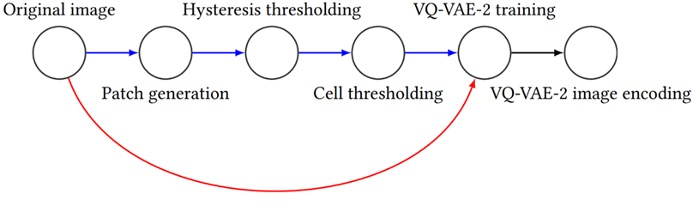
\includegraphics[width=1\linewidth]{Figures/Overview VQVAE pipeline.jpeg}
\captionof{figure}{Figure caption}
\end{center}

\paragraph{Data preprocessing:}
	Extract tiles from the Camelyon 2016 subset dataset
	Select tiles containing tissue samples via hysteresis thresholding
\paragraph{VQVAE training:}
	Train VQVAE at three compression ratios (~4.8, ~9.8 and ~19.2) on Camelyon 2016 subset thresholded tiles for 500 epochs for each model.
	Train VQVAE at three compression ratios (~4.8, ~9.8 and ~19.2) on the thresholded Camelyon 2016 patches for 500 epochs, while using a custom data augmentation method which randomises channels to increase model generalisability and transferability.
\paragraph{VQVAE testing:}
	Test trained VQVAEs on the Camelyon 2016 subset, UCLA and Internal Validation set.
	Test VQVAEs with data augmented training data on the Camelyon 2016 subset, UCLA and Internal Validation set.
	Analyse generated metrics (SSIM, PSNR, SSIM per Compression ratio and PSNR per Compression ratio)
\paragraph{JPEG compression testing:}
	Test JPEG compression ratios (2 to 97 with intervals of 5) for JPEG and JPEG 2000 compression with and without metadata removed using the --strip function.
	Analyse the generated metrics (SSIM, PSNR, SSIM per Compression ratio and PSNR per Compression ratio).

\subsection{Datasets}
\paragraph{Camelyon 2016 subset:} Camelyon was created for cancer segmentation and classification tasks on digital pathology whole slide images. Originally presented in the Camelyon challenge. The Camelyon dataset was created for two years, creating the Camelyon 2016 dataset (n=170 WSIs), and the Camelyon 2017 dataset. The Camleyon 2016 dataset is from two hospitals, whereas Camelyon 2017 is from five hospitals. For preliminary experiments on the networks, a subset of the Camelyon 2016 dataset was used, containing Normal slides 1-10 (excluding 9) and Cancerous slides (1-10). These WSIs were converted to smaller patches for network training and testing.

\paragraph{UCLA:} The UCLA dataset (n=21 benign, 21 malignant) is a dataset from the University of California. UCLA consists of WSI slide scans, mainly of breast cancer tissue.

\paragraph{Internal validation set:} This was a dataset used for internal validation of the algorithms and testing. The internal validation set consisted of 8,455 512x512x3 patches, which after thresholding was applied became 1,935 512x512x3 patches containing tissue. This dataset allows for testing the models on images from real world data, containing image artefacts.

\subsection{Data preprocessing}
\paragraph{WSI patch extraction:} OpenSlide was used to extract patches, these patches were 512x512x3 with an overlap of 0. We then used the Scikit-image hysteresis thresholding implementation to create a hysteresis threshold map. The hysteresis threshold map was then used to measure the amount of tissue within the patch, with any patch that was over 10\% of the slide being tissue being placed into a thresholded patch set for model training.

\paragraph{Data Augmentation:} Data augmentation was used on the training image patches (X) in the form of torchvision.transforms.Compose([torchvision.transforms.Resize((512, 512)), torchvision.transforms.toTensor()]).A custom colour randomising algorithm was also used during VQVAE training, this used a Image:x_ijk↦U~(0,2)*(x_ijk )  | k∈{0,1,2}.

\begin{center}
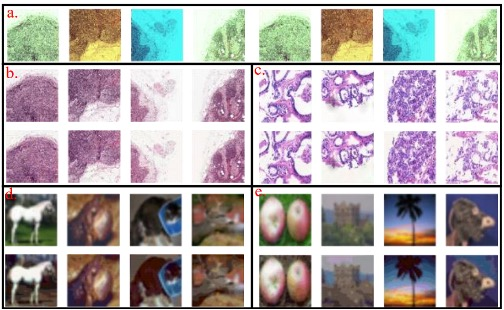
\includegraphics[width=1\linewidth]{Figures/Example VQVAE images reconstructions and data augmentation.jpeg}
\captionof{figure}{Figure caption}
\end{center}

% Figure 1. a. shows example Camelyon 2016 subset training images with the colour augmentation applied to the training patches. Figure 1. b. shows the same training image batch without image the data augmentation applied and the reconstruction with the Camelyon 2016 trained VQVAE. Figure 1. c. d. e, show the original and reconstructed testing patches for the UCLA, Cifar 10 and Cifar 100 datasets.

\subsection{Algorithms}
\paragraph{VQVAE architecture:} The VQVAE architecture uses an encoder, a decoder and a quantizer. The VQVAE2 modified this with a secondary encoder and decoder layer. The secondary (top) and primary (bottom) encoder and decoder layers encode for high level and low-level features within the image respectively.

\begin{center}
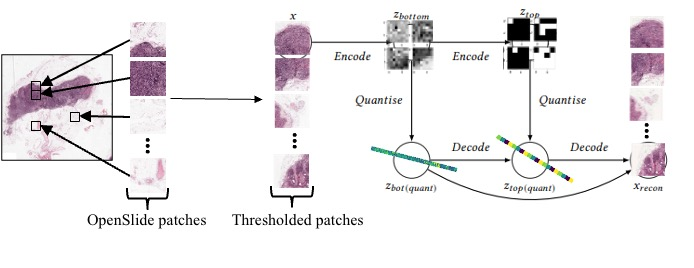
\includegraphics[width=1\linewidth]{Figures/Overview diagram VQVAE patch extraction and algorithm.jpeg}
\captionof{figure}{Figure caption}
\end{center}
    
\paragraph{Loss function:} The loss function within the VQVAE has three components, the reconstruction loss, the embedding loss and the commitment loss. The reconstruction loss encodes for the accuracy of the reconstructed image (X') and can be any existing loss function including the mean squared error (MSE). The embedding loss moves the code book embeddings (Zembed(X)) towards the normal distribution quantised embeddings (Zembed(quant)). The commitment loss moves the embedding (Zembed(quant)) towards the image encoded embedding (Zembed(X)).
    VQVAE loss=Reconstruction loss+embedding loss-commitment loss
    VQVAE loss=MSE(X,X')+(Z_(embed(X))-Z_embed(quant)  )-β(Z_embed(quant) -Z_(embed(X)) )
    
\paragraph{VQVAE training:} The VQVAE implementation was cloned from the GitHub repository (https://github.com/rosinality/vq-vae-2-pytorch). The default parameters were used for initial training and preliminary testing. The dimension of embeddings and number of embedding parameters were modified to achieve larger or smaller compression of the 512x512x3 image patches. The VQVAE was trained on the Camelyon 2016 subset training data, and then was tested on all other datasets. \\
The default VQVAE network parameters (in_channel=3, channel=128, n_res_block=2, n_res_channel=32, embed_dim=64, n_embed=512, decay=0.99, loss_function=LossFunction.mean_squared_error) led to a compression ratio of 0.6. The embedding dimension parameter can be changed to change the level of compression within the compressed representation. The embedding dimensions for the embed_dim values of 8, 4, 2 are 4.8:1, 9.8:1 and 19.2:1 respectively for the compression ratio between the compressed representation (X^') and the original patch image (X). For example within the training within this paper the embedding dimension value of 2 was used to create a 19.2:1 compression ratio with a R^((2,128,128) )+R^((2,64,64) ) latent space for the R^((512,512,3) ) image data (X).

\begin{equation}
    X\in\mathbb{R}^{(512, 512, 3)};\\ X^{quant\_t}\in\mathbb{R}^{(embed_dim, 128, 128)}; X^{quant\_b}\in\mathbb{R}^{(embed_dim, 64, 64)}; X'\in\mathbb{R}^{(512, 512, 3)}
\end{equation}
    
\begin{align*}
    encode: X\mapsto (X^{quant\_t}\union X^{quant\_b}) \\
    decode: (X^{quant\_t}, X^{quant\_b}\mapsto X') \\
    VQVAE(X): decode(encode(X))\mapsto X'
    \label{eq:VQVAEarchitecture}
\end{align*}

    % X∈R^((512,512,3) );X^(quant\_t)∈R^((embed\_dim,128,128) );X^(quant\_b)∈R^((embed\_dim,64,64) );X^'∈R^((512,512,3) ) \\
    % encode: X→〖(X〗^(quant\_t)∪X^(quant\_b)) \\
    % decode: (X^(quant\_t),X^(quant\_b) )→X^' \\
    % VQVAE(X):decode(encode(X))→X^' \\
    
\paragraph{JPEG:} Two ImageMagick JPEG implementations were used: the generic JPEG implementation (“magick {source_file} -strip -quality {quality} {result_file}”), 
 and the JPEG 2000 compression (magick {source_file} -strip -colorspace RGB -define jp2:quality {compression ratio} {result_file}”. \\
 All JPEG compression algorithms were run on the same datasets to the VQVAE, using the same Pytorch dataloaders without data augmentation other than “torchvision.transforms.Resize((512, 512))” for all patches within the pathology datasets. \\
 The JPEG compression algorithm compression quality metric was used for every 5\% quality from 2\% to 99\%, this was manually mapped to the compression ratio of the compressed representation. The JPEG 2000 used the same numbers from 2 to 99 but within JPEG 2000 this value represented the desired compression ratio. The PSNR and SSIM values were calculated for all reconstructed images and plotted as a function of the compression ratio for both the JPEG and JPEG 2000 algorithms.

\section{Results}
\paragraph{Visual differences between JPEG and VQVAE compression:} JPEG and JPEG 2000 are current compression techniques used within WSI storage within hospitals. The compression ratio within these stored images is usually around 15:1 to 20:1 compression ratio. The VQVAE trained on a 19.2:1 compression ratio reconstructed images were then visually compared to the decompressed images from the JPEG compression testing. \\
The reconstructions seemed to be performing better on all datasets compared to the JPEG compression at a similar compression level. \\
\paragraph{Custom data augmentation (colour randomisation):} The custom colour augmented dataset performed worse in all metrics compared to the VQVAE trained without the custom data augmentation. The difference in PSNR (mean [standard deviation]) between the VQVAE trained to the compression ratio of ~19.2 was 1.22 [0.17], -2.2 [0.59], 1.13 [0.42] for the mean and standard deviations of 19.92±1.83, 20.09±1.29, 21.95±1.89 (no colour data augmentation) and 18.70±1.66, 22.29±0.70, 20.82±1.47 (with randomised colour data augmentation) for the Camelyon 2016 subset, UCLA and Internal validation set. The difference in the SSIM for the VQVAE trained to the compression ratio of ~19.2 was 0.11 [-0.024], 0.03 [-0.001], 0.07 [-0.009] from the mean and standard deviation of 0.72±0.076, 0.88±0.018, 0.80±0.060 (no colour data augmentation) and 0.61±0.10, 0.85±0.019, 0.73±0.069 (with randomised colour data augmentation) for the Camelyon 2016 subset, UCLA and Internal validation set respectively. \\
The difference within the median and IQR values for the different algorithms can be seen within following boxplots.

\paragraph{JPEG compression quality quantitative results:} The peak signal to noise ratio (PSNR) and structural similarity (SSIM) JPEG metrics were calculated for the JPEG compression. The PSNR for JPEG on the tested pathology datasets dropped significantly from 43 to 32 between the 1:1 and 3:1 compression ratios. The PSNR for JPEG maintained stable with a PSNR of around 29 after the 5:1 compression ratio.

\begin{center}
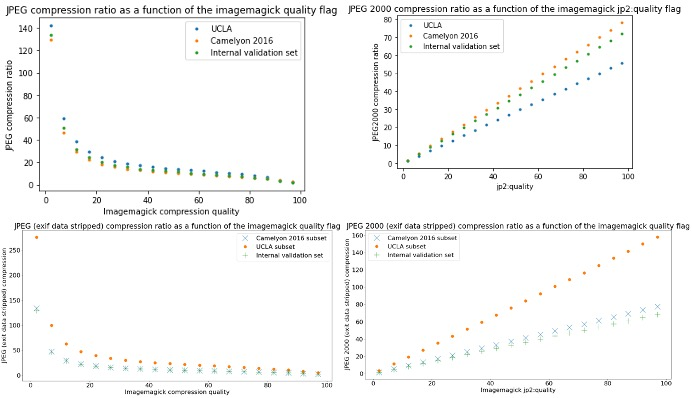
\includegraphics[width=1\linewidth]{Figures/JPEG ImageMagick compression quality to compression ratio with and without metadata.jpeg}
\captionof{figure}{Figure caption}
\end{center}

\paragraph{JPEG vs VQVAE (mean and standard deviation):} The PSNR (PSNR∈R) mean and standard deviation for the UCLA and Camelyon 2016 subset with metadata were 28 dB and 28.75 dB. The PSNR for the UCLA, Camelyon 2016 subset and internal validation set with exif data stripped with imagemagicks -strip flag were 31.50±0.81 dB, 29.70±1.28 dB, 29.91±1.21 dB for the compression ratio of ~19.2:1 for JPEG compression. For the VQVAE compression the PSNRs mean and standard deviation were 20.3±1.09 dB, 19.6 ± 1.77 dB, 21.49 ± 1.83 dB, respectively. Structural Similarity (SSIM) considers image structure, PSNR does not. SSIM (SSIM∈[0,1]) results for the UCLA, Camelyon 2016 subset and internal validation set were 0.35, 0.35 for JPEG with exif data. Without exif data (imagemagick –strip flag) the UCLA, Camelyon 2016 subset and internal validation set SSIM mean and standard deviation was 0.84 ± 0.022, 0.83 ± 0.034, 0.80 ± 0.042 for JPEG and 0.85 ± 0.022, 0.72 ± 0.072, 0.79 ± 0.056 for the VQVAE implementation.

\begin{center}
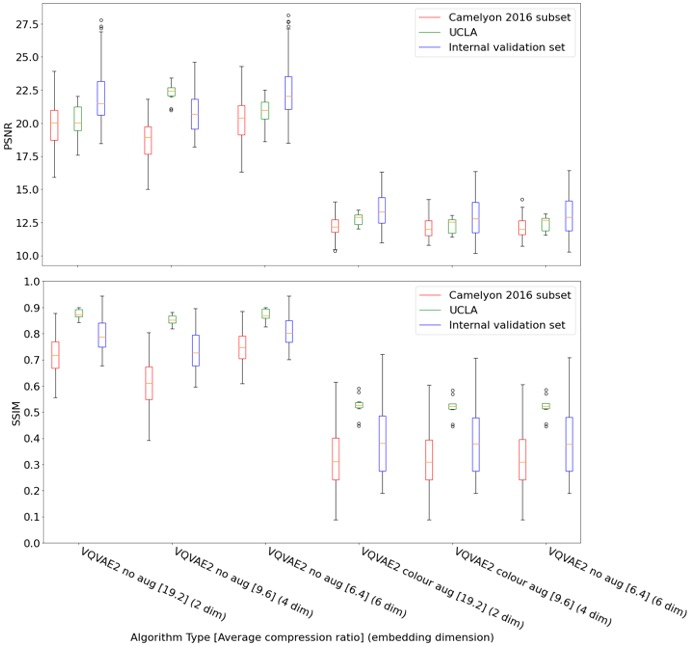
\includegraphics[width=1\linewidth]{Figures/VQVAE data augmentation PSNR SSIM comparison boxplot.jpeg}
\captionof{figure}{Figure caption}
\end{center}

\paragraph{19.5:1 JPEG vs 19.2:1 (VQVAE medium and interquartile range):} The PSNR medium and interquartile range for the UCLA and Camelyon 2016 subset and internal validation set are ~21, 20, 21 and ~32, 29, 30 for the VQVAE and JPEG respectively.
The SSIM medium and interquartile range for the UCLA and Camelyon 2016 subset and internal validation set are ~0.85, 0.72, 0.79 and ~0.84, 0.81, 0.8 for the VQVAE and JPEG respectively.

\begin{center}
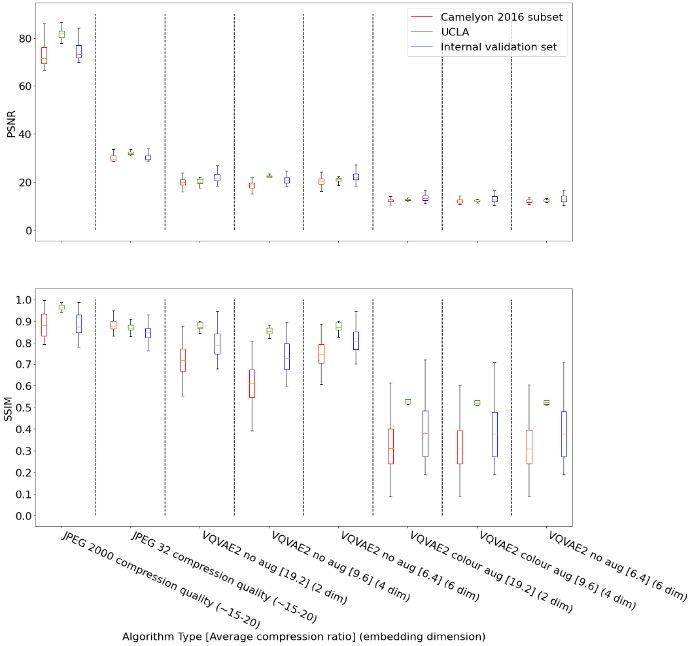
\includegraphics[width=1\linewidth]{Figures/VQVAE data augmentation PSNR SSIM comparison boxplot With JPEG and JPEG 2000.jpeg}
\captionof{figure}{Figure caption}
\end{center}
 
\section{Discussion}
The quantitative metrics for the initial VQVAE testing showed that the VQVAE could perform to a degree that was, on average, either comparable or better than JPEG within the SSIM metric, but worse on the PSNR metric if JPEG metadata is saved. If this is removed the VQVAE SSIM is lower than that of JPEG and JPEG 2000. \\
The PSNR does not consider structural similarity of the two images, the structural similarity (SSIM) metric does consider the similarity of the structures within the image. 
VAEs and VQVAEs have been used successfully for compression and meaning representation tasks within other clinical domains, including within x-ray and CT compression [9]. \\
As the learnt model was able to generalise between different scanners and different datasets from different locations, the latent space was shown to encode features that represented the image features within the image. Future work aims to understand the representations generated by Variational Autoencoder networks, aiming to create clinically useful representations of WSI slides and patches while allowing for compression of the pathology images. \\
\paragraph{Limitations:} The tested variational autoencoder networks may have been mapping too much towards the reconstructed image, rather than ensuring mapping to the normal distribution feature representations, therefore ignoring the normal distribution feature mapping in favour of minimizing the reconstruction image accuracy, latent space testing and visualisation is aimed to be done in the future. \\
The poorer results for the VQVAE2 implementation on the PSNR could have been down to a lack of training of the model (epochs=500), however training new models on 2000 epochs did not change the results significantly. The poorer results for the VQVAE implementation versus the JPEG implementations could also have been due to the use of suboptimal training hyper parameters, or possibly the use of a loss function that did not focus on the image reconstruction quality, with the latent space embedding representations being favoured or balanced over the reconstruction accuracy metrics of PSNR or SSIM. \\
A full hyperparameter search for the VQVAE network was not performed to gain the optimal parameters for the network compression. \\
More WSI slides could have been used for training and testing of the data, using multiple datasets should mitigate the generalisability of this issue. As the metrics were done on a per patch basis, this may not be fully transferable to a whole slide image compression metric, further research would have to be done to confirm this. \\
\paragraph{Future work:} Future research could focus on merging of the data with VAEs and other techniques, for example, normalizing flows and manifolds. \\
If the compression of VAEs could compete with existing methods, the compression would allow for the compressed representation to contain meaning within the latent features, possibly allowing for abstraction of clinically relevant features for clinicians to use for faster analysis of the biopsy tissue contained on the slide. \\
Future research aims to compare the compression error type to subjective image quality and performance metrics. \\

\section{Compliance with Ethical Standards}
This work was performed as part of ethical approval given within the NPIC NHS ethical approval REC 05/Q1205/220 which covers future work to analyses digital pathology images.
All used internal validation datasets were anonymized before use and were used in secure computing environments. All slides were kept in accordance with Leeds university and NHS guidelines. 

\section{Acknowledgements}
Jason Keighley is funded via the Leeds University CDT for AI in medical diagnosis and care. Marc de Kamps is a lecturer at the school of computing at the university of Leeds. Alex Wright is a member of NPIC within LTHT and is working on digitization of LTHT patient pathology slides. \\
Support was provided by National Pathology Imaging Co-operative, NPIC (Project no. 104687), supported by a £50m investment from the Data to Early Diagnosis and Precision Medicine strand of the government’s Industrial Strategy Challenge Fund, managed and delivered by UK Research and Innovation (UKRI). \\

\section{References}



% \section{The Elsevier article class}

% \paragraph{Installation} If the document class \emph{elsarticle} is not available on your computer, you can download and install the system package \emph{texlive-publishers} (Linux) or install the \LaTeX\ package \emph{elsarticle} using the package manager of your \TeX\ installation, which is typically \TeX\ Live or Mik\TeX.

% \paragraph{Usage} Once the package is properly installed, you can use the document class \emph{elsarticle} to create a manuscript. Please make sure that your manuscript follows the guidelines in the Guide for Authors of the relevant journal. It is not necessary to typeset your manuscript in exactly the same way as an article, unless you are submitting to a camera-ready copy (CRC) journal.

% \paragraph{Functionality} The Elsevier article class is based on the standard article class and supports almost all of the functionality of that class. In addition, it features commands and options to format the
% \begin{itemize}
% \item document style
% \item baselineskip
% \item front matter
% \item keywords and MSC codes
% \item theorems, definitions and proofs
% \item lables of enumerations
% \item citation style and labeling.
% \end{itemize}

% \section{Front matter}

% The author names and affiliations could be formatted in two ways:
% \begin{enumerate}[(1)]
% \item Group the authors per affiliation.
% \item Use footnotes to indicate the affiliations.
% \end{enumerate}
% See the front matter of this document for examples. You are recommended to conform your choice to the journal you are submitting to.

% \section{Bibliography styles}

% There are various bibliography styles available. You can select the style of your choice in the preamble of this document. These styles are Elsevier styles based on standard styles like Harvard and Vancouver. Please use Bib\TeX\ to generate your bibliography and include DOIs whenever available.

% Here are two sample references: \cite{Feynman1963118,Dirac1953888}.

\nocite{*}

\bibliography{references.bib}

\end{document}